%=====================================================================
%  We Know Group | FreedomPay Windows FCC Integration Guide
%  Auth & Capture  --  Version 2.0 (July 2026)
%
%  Branding per "We Know Group Brand Guidelines V2 2023":
%    - Primary colours: Graphite #121212, Azure #00A6D3, White
%    - Secondary: Sky Blue #E5F1F9, Sea Blue #008BB2, Night Blue #0C2752
%    - Greys: Night #575A5C, Mid #ADADAD, Light #F4F4F4
%    - Typeface: Circular Pro (approximated here with Inter, the licensed
%      brand stand-in used in the WeKnow Employee Handbook)
%    - Logos are the official WeKnow assets in images/ -- never redrawn.
%
%  Screenshots in images/ are sourced from the certified WeKnow "Windows
%  FCC - Auth & Capture" submission; sensitive values are pre-redacted.
%  Structure follows FreedomPay "FCC Card Present Documentation Example".
%=====================================================================
\documentclass[a4paper,10pt]{article}

%---------------------------------------------------------------------
% Fonts & encoding -- Inter (brand stand-in for Circular Pro)
%---------------------------------------------------------------------
\usepackage[T1]{fontenc}
\usepackage[utf8]{inputenc}
\usepackage[sfdefault]{inter}
\renewcommand{\familydefault}{\sfdefault}
\usepackage{microtype}

%---------------------------------------------------------------------
% Layout
%---------------------------------------------------------------------
\usepackage[a4paper,margin=20mm,top=28mm,bottom=22mm,headheight=20pt,headsep=14pt]{geometry}
\usepackage{graphicx}
\graphicspath{{images/}}
\usepackage[table]{xcolor}
\usepackage{tikz}
\usetikzlibrary{arrows.meta,positioning,calc,shapes.misc,fit,backgrounds}
\usepackage{tcolorbox}
\tcbuselibrary{skins,breakable}
\usepackage{booktabs}
\usepackage{array}
\usepackage{longtable}
\usepackage{tabularx}
\usepackage{enumitem}
\usepackage{fancyhdr}
\usepackage{titlesec}
\usepackage{listings}
\usepackage{float}
\usepackage{lastpage}
\usepackage{amssymb}
\usepackage{caption}
\usepackage[hidelinks,colorlinks=true,urlcolor=weknowsea,linkcolor=weknownight]{hyperref}

%---------------------------------------------------------------------
% We Know Group palette (Brand Guidelines V2 2023, Section 3)
%---------------------------------------------------------------------
\definecolor{weknowazure}{HTML}{00A6D3}     % Hero colour
\definecolor{weknowgraphite}{HTML}{121212}
\definecolor{weknowsky}{HTML}{E5F1F9}
\definecolor{weknowsea}{HTML}{008BB2}
\definecolor{weknownight}{HTML}{0C2752}
\definecolor{weknowgreyN}{HTML}{575A5C}
\definecolor{weknowgreyM}{HTML}{ADADAD}
\definecolor{weknowgreyL}{HTML}{F4F4F4}

%---------------------------------------------------------------------
% Headers / footers -- thin ruled band, real logo top-right
%---------------------------------------------------------------------
\pagestyle{fancy}
\fancyhf{}
\fancyhead[L]{\footnotesize\color{weknowgreyN}\nouppercase{\leftmark}}
\fancyhead[R]{\raisebox{-0.35\height}{
\includegraphics[height=15pt]{wkg-logo-horizontal}}}
\renewcommand{\headrulewidth}{0.4pt}
\renewcommand{\headrule}{\hbox to\headwidth{\color{weknowgreyM}\leaders\hrule height \headrulewidth\hfill}}
\fancyfoot[L]{\scriptsize\color{weknowgreyN}Confidential --- We Know Group}
\fancyfoot[C]{\scriptsize\color{weknowgreyN}FreedomPay Windows FCC --- Auth \& Capture}
\fancyfoot[R]{\scriptsize\color{weknowgreyN}Page \thepage\ of \pageref{LastPage}}
\renewcommand{\footrulewidth}{0.4pt}
\renewcommand{\footrule}{\hbox to\headwidth{\color{weknowgreyM}\leaders\hrule height \footrulewidth\hfill}}

%---------------------------------------------------------------------
% Section styling
%---------------------------------------------------------------------
\titleformat{\section}
  {\color{weknownight}\LARGE\bfseries}
  {\thesection}{0.7em}{}
\titleformat{\subsection}
  {\color{weknowsea}\Large\bfseries}
  {\thesubsection}{0.6em}{}
\titleformat{\subsubsection}
  {\color{weknowgraphite}\large\bfseries}
  {\thesubsubsection}{0.6em}{}
\titlespacing*{\section}{0pt}{20pt}{10pt}
\titlespacing*{\subsection}{0pt}{16pt}{6pt}
\titlespacing*{\subsubsection}{0pt}{12pt}{4pt}
\renewcommand{\sectionmark}[1]{\markright{\thesection\quad #1}}

%---------------------------------------------------------------------
% Captions -- numbered figures, subtle brand styling
%---------------------------------------------------------------------
\captionsetup{font=small,labelfont={bf,color=weknownight},
              textfont={color=weknowgreyN},skip=5pt}

%---------------------------------------------------------------------
% Screenshot helper -- bordered, centred, floated in place (no overlap)
%   \screenshot[width fraction]{file}{caption}
%---------------------------------------------------------------------
\newcommand{\screenshot}[3][0.82]{%
  \begin{figure}[H]
    \centering
    \setlength{\fboxsep}{0pt}\setlength{\fboxrule}{0.6pt}%
    {\color{weknowgreyM}\fbox{\includegraphics[width=#1\linewidth]{#2}}}%
    \caption{#3}
  \end{figure}}

%---------------------------------------------------------------------
% Callout boxes
%---------------------------------------------------------------------
\newtcolorbox{wkinfo}[1][]{%
  enhanced,breakable,colback=weknowsky,colframe=weknowazure,
  boxrule=0pt,leftrule=2.5pt,arc=1.5pt,
  fonttitle=\bfseries,coltitle=weknownight,title={#1},
  left=6pt,right=6pt,top=5pt,bottom=5pt}
\newtcolorbox{wkwarn}[1][]{%
  enhanced,breakable,colback=weknowgreyL,colframe=weknownight,
  boxrule=0pt,leftrule=2.5pt,arc=1.5pt,
  fonttitle=\bfseries,coltitle=weknownight,title={#1},
  left=6pt,right=6pt,top=5pt,bottom=5pt}

%---------------------------------------------------------------------
% Code listings (config snippets)
%---------------------------------------------------------------------
\lstdefinestyle{wkxml}{
  basicstyle=\ttfamily\footnotesize\color{weknowgraphite},
  backgroundcolor=\color{weknowgreyL},
  frame=single, framerule=0pt, rulecolor=\color{weknowgreyL},
  breaklines=true, breakatwhitespace=false,
  columns=fullflexible, keepspaces=true,
  aboveskip=8pt, belowskip=8pt, xleftmargin=6pt, framexleftmargin=6pt}
\lstset{style=wkxml}

\newcolumntype{L}[1]{>{\raggedright\arraybackslash}p{#1}}
\setlist{nosep,itemsep=3pt}

\begin{document}

%=====================================================================
% COVER  (FreedomPay example layout, WeKnow brand: azure hero band,
%         white title, real horizontal logo on the white lower band)
%=====================================================================
\begin{titlepage}
\thispagestyle{empty}
\begin{tikzpicture}[remember picture,overlay]
  % Azure hero band across the top ~62% of the page
  \fill[weknowazure]
    (current page.north west) rectangle
    ([yshift=-185mm]current page.north east);
  % Night-blue baseline accent under the band
  \fill[weknownight]
    ([yshift=-185mm]current page.north west) rectangle
    ([yshift=-188mm]current page.north east);
  % Headline -- white on azure
  \node[anchor=north west,text=white,align=left,font=\bfseries]
    at ([xshift=20mm,yshift=-52mm]current page.north west)
    {\fontsize{36}{42}\selectfont FreedomPay\\[3pt]Windows FCC};
  \node[anchor=north west,text=white,align=left]
    at ([xshift=20mm,yshift=-118mm]current page.north west)
    {\fontsize{18}{24}\selectfont Auth \& Capture Integration Guide};
  % Version block -- graphite on white
  \node[anchor=north west,align=left,text=weknowgraphite]
    at ([xshift=20mm,yshift=-205mm]current page.north west)
    {{\Large\bfseries Version 2.0}\\[4pt]
     {\normalsize\color{weknownight}July 2026}\\[2pt]
     {\small\color{weknowgreyN}We Know Group --- Internal Implementation \& Support Documentation}};
  % Official WeKnow logo -- bottom-left, on the white band
  \node[anchor=south west]
    at ([xshift=20mm,yshift=22mm]current page.south west)
    {
\includegraphics[width=48mm]{wkg-logo-horizontal}};
  % Provenance -- bottom-right
  \node[anchor=south east,text=weknowgreyN,font=\footnotesize,align=right]
    at ([xshift=-20mm,yshift=24mm]current page.south east)
    {Prepared for FreedomPay certification\\
     per Certification Documentation Requirements Guide v1.9\\[2pt]
     www.WeKnowLondon.com};
\end{tikzpicture}
\end{titlepage}

%=====================================================================
% VERSION HISTORY
%=====================================================================
\section*{Document Version History}
\begin{center}
\renewcommand{\arraystretch}{1.35}
\begin{tabularx}{\textwidth}{L{16mm} L{24mm} L{34mm} X}
\rowcolor{weknownight}\color{white}\textbf{Version} &
\color{white}\textbf{Date} & \color{white}\textbf{Author} &
\color{white}\textbf{Reason for Change}\\
2.0 & 2026-07-10 & WeKnow Integrations &
Full refresh against docs.freedompay.com: updated UAT/Production
IP ranges and domain allow-lists, FCC 5.4.x configuration keys
(\texttt{BinMap2.txt}, AMA v2 endpoints), Standalone installer flow
with Remote Update Service, current error-code tables, FreedomPay
L2 support contacts and SLAs, and new data-flow diagrams.\\
\rowcolor{weknowgreyL}
1.x & 2024 & WeKnow Integrations &
Initial Windows FCC Auth \& Capture documentation set
(FCC 5.3.2.15 baseline).\\
\end{tabularx}
\end{center}

\begin{wkinfo}[Scope]
This guide covers the \textbf{Windows FCC} integration only, deployed in
\textbf{standalone} mode (FCC Server Service and FCC Client Service on the
same workstation as the WeKnow SSM POS client). Certified transaction
types: \textbf{Auth} (card present and card not present) and
\textbf{Capture} with follow-on incremental authorisations. Always confirm
the latest endpoint and configuration details against the FreedomPay
documentation portal at \url{https://docs.freedompay.com/fcc/welcome/readme}.
\end{wkinfo}

\tableofcontents
\clearpage

%=====================================================================
% 1  OVERVIEW
%=====================================================================
\section{Overview}

Connecting FreedomPay as the payment gateway in WeKnow uses FreedomPay's
\textbf{Freeway Commerce Connect (FCC)} middleware. FCC consists of two
lightweight Windows services that coordinate the flow of data between the
WeKnow SSM application and the Point of Interaction (POI) pin-pad
terminal:

\begin{center}
\renewcommand{\arraystretch}{1.3}
\begin{tabularx}{\textwidth}{L{32mm} L{30mm} X}
\rowcolor{weknownight}\color{white}\textbf{Windows Service} &
\color{white}\textbf{Role} & \color{white}\textbf{Primary responsibility}\\
FCC Server & The logic engine &
Entry point for the WeKnow (SSM) POS application. Receives the
\texttt{POSRequest}, handles request routing and decision logic, and
returns the \texttt{POSResponse}.\\
\rowcolor{weknowgreyL}
FCC Client & The device handler &
Directly manages the POI device: wakes the device, drives the customer
interaction, and captures encrypted card data.\\
\end{tabularx}
\end{center}

We deploy FCC in \textbf{standalone} configuration
(\texttt{operationMode="standalone"}): the FCC Server Service and the FCC
Client Service reside on the same workstation as the WeKnow SSM POS
client. All payment processing occurs securely in \textbf{Freeway},
FreedomPay's cloud gateway, over HTTPS (TLS 1.2 or higher) with encrypted
data returned to WeKnow. Card data is encrypted at the POI device and is
never available in cleartext to WeKnow.

%=====================================================================
% 2  DATA FLOW DIAGRAMS
%=====================================================================
\section{Data Flow Diagram(s)}

\subsection{System topology (standalone)}

\begin{figure}[H]
\centering
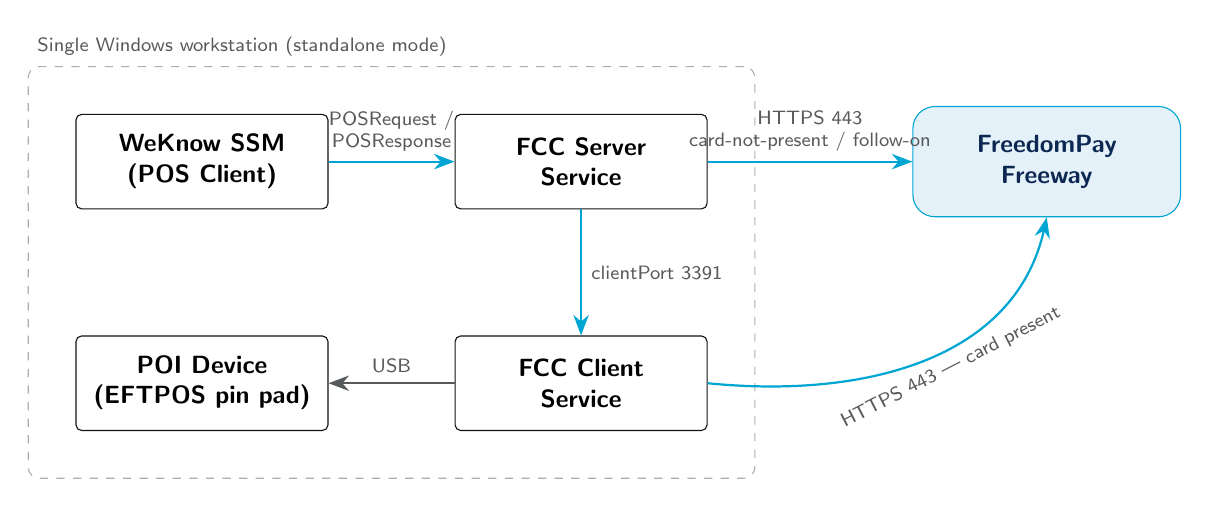
\begin{tikzpicture}[
  node distance=10mm and 16mm,
  box/.style={draw=weknowgraphite,fill=white,rounded corners=2pt,
              minimum width=32mm,minimum height=12mm,align=center,
              font=\small\bfseries},
  cloud/.style={draw=weknowazure,fill=weknowsky,rounded corners=8pt,
              minimum width=34mm,minimum height=14mm,align=center,
              font=\small\bfseries,text=weknownight},
  lbl/.style={font=\scriptsize,text=weknowgreyN},
  arr/.style={-{Stealth[length=2.6mm]},thick,weknowazure},
  arrg/.style={-{Stealth[length=2.6mm]},thick,weknowgreyN}]

  \node[box] (ssm) {WeKnow SSM\\(POS Client)};
  \node[box,right=of ssm] (server) {FCC Server\\Service};
  \node[box,below=16mm of server] (client) {FCC Client\\Service};
  \node[box,left=of client] (poi) {POI Device\\(EFTPOS pin pad)};
  \node[cloud,right=26mm of server] (freeway) {FreedomPay\\Freeway};

  \begin{scope}[on background layer]
    \node[draw=weknowgreyM,dashed,rounded corners=4pt,inner sep=6mm,
          fit=(ssm)(server)(client)(poi),
          label={[lbl,anchor=south west]north west:
          Single Windows workstation (standalone mode)}] {};
  \end{scope}

  \draw[arr] (ssm) -- node[lbl,above,align=center]{POSRequest /\\POSResponse} (server);
  \draw[arr] (server) -- node[lbl,right]{clientPort 3391} (client);
  \draw[arrg] (client) -- node[lbl,above]{USB} (poi);
  \draw[arr] (server) -- node[lbl,above,align=center]{HTTPS 443\\card-not-present / follow-on} (freeway);
  \draw[arr] (client.east) .. controls +(20mm,-2mm) and +(-4mm,-18mm) ..
             node[lbl,below,sloped,pos=0.55]{HTTPS 443 --- card present}
             (freeway.south);
\end{tikzpicture}
\caption{Standalone topology: both FCC services and the WeKnow SSM client run on one workstation; all gateway traffic is HTTPS to Freeway.}
\end{figure}

\subsection{Card payment --- AUTH (swiped, tapped, keyed or inserted)}

\begin{figure}[H]
\centering
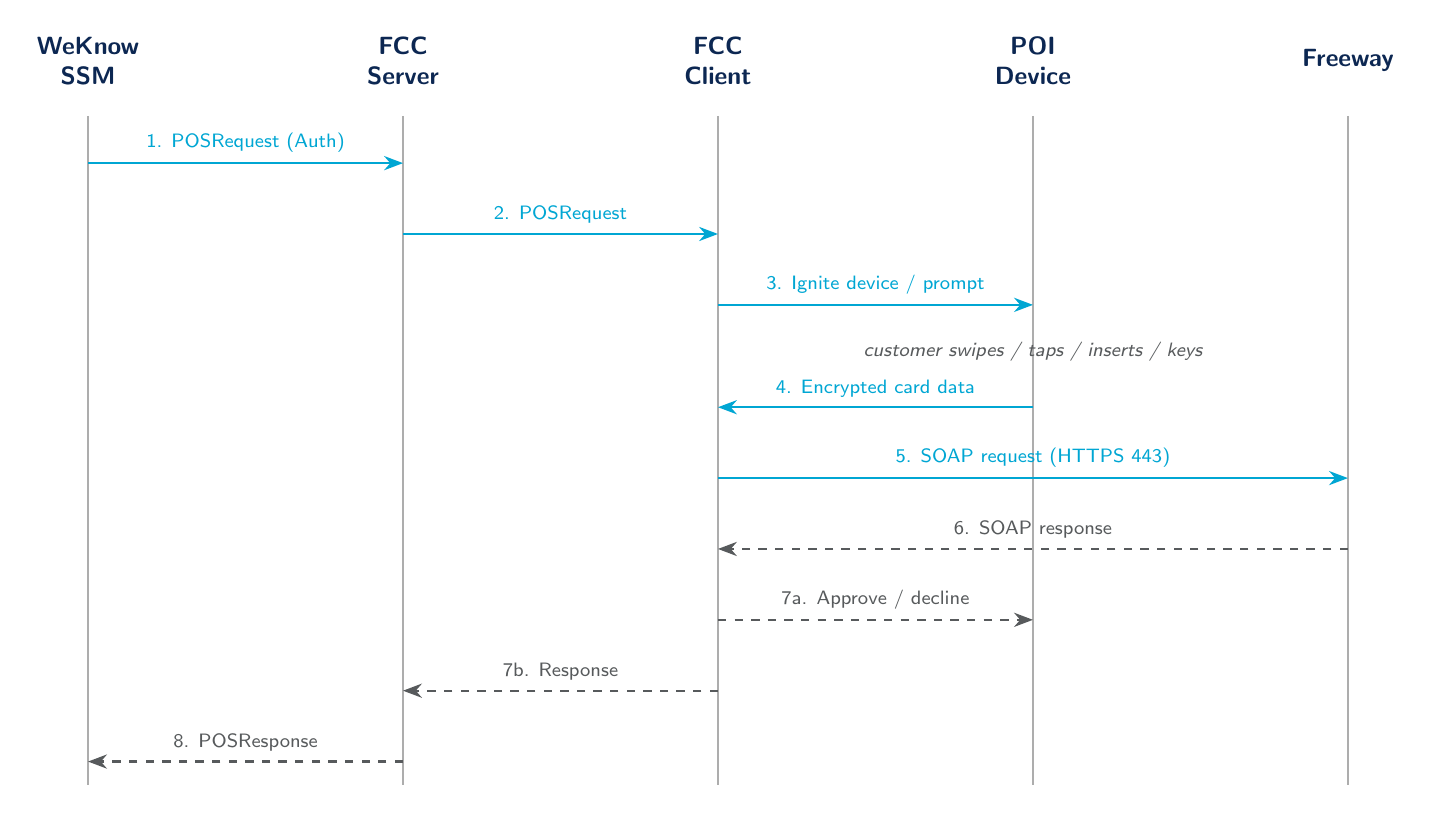
\begin{tikzpicture}[
  lane/.style={font=\small\bfseries,text=weknownight,align=center},
  life/.style={weknowgreyM,thick},
  msg/.style={-{Stealth[length=2.4mm]},thick,weknowazure,font=\scriptsize},
  ret/.style={-{Stealth[length=2.4mm]},thick,dashed,weknowgreyN,font=\scriptsize}]
  % lifelines -- evenly spaced, generous gaps so labels never touch a line
  \foreach \x/\name/\txt in {0/ssm/{WeKnow\\SSM}, 4/srv/{FCC\\Server},
                             8/cli/{FCC\\Client}, 12/poi/{POI\\Device},
                             16/fwy/Freeway}{
    \node[lane] (\name) at (\x,0) {\txt};
    \draw[life] (\x,-0.7) -- (\x,-9.2);}
  % messages -- one clear step per row
  \draw[msg] (0,-1.3)  -- node[above]{1. POSRequest (Auth)} (4,-1.3);
  \draw[msg] (4,-2.2)  -- node[above]{2. POSRequest} (8,-2.2);
  \draw[msg] (8,-3.1)  -- node[above]{3. Ignite device / prompt} (12,-3.1);
  \node[font=\scriptsize\itshape,text=weknowgreyN] at (12,-3.7)
       {customer swipes / taps / inserts / keys};
  \draw[msg] (12,-4.4) -- node[above]{4. Encrypted card data} (8,-4.4);
  \draw[msg] (8,-5.3)  -- node[above]{5. SOAP request (HTTPS 443)} (16,-5.3);
  \draw[ret] (16,-6.2) -- node[above]{6. SOAP response} (8,-6.2);
  \draw[ret] (8,-7.1)  -- node[above]{7a. Approve / decline} (12,-7.1);
  \draw[ret] (8,-8.0)  -- node[above]{7b. Response} (4,-8.0);
  \draw[ret] (4,-8.9)  -- node[above]{8. POSResponse} (0,-8.9);
\end{tikzpicture}
\caption{Card-present Auth message sequence between WeKnow SSM, the FCC services, the POI device and Freeway.}
\end{figure}

\begin{enumerate}
  \item WeKnow (SSM) sends the Auth \texttt{POSRequest}
        (keyed / swiped / tapped / inserted) to the FCC Server Service.
  \item The FCC Server Service forwards the \texttt{POSRequest} to the
        FCC Client Service. (If the request already contains card data,
        the FCC Server sends it directly to Freeway instead --- see
        \S\ref{sec:cnp}.)
  \item The FCC Client Service ignites the POI device; the customer
        interacts with the device.
  \item The POI device encrypts the card data and sends it to the FCC
        Client Service.
  \item The FCC Client Service sends the SOAP request to Freeway over
        HTTPS (port 443, TLS 1.2+).
  \item Freeway processes the transaction with the processor and returns
        the SOAP response to the FCC Client Service.
  \item The FCC Client Service returns the result to the POI device
        (displays approve or decline) and forwards the response to the
        FCC Server Service.
  \item The FCC Server Service returns the \texttt{POSResponse} to
        WeKnow (SSM).
\end{enumerate}

\subsection{Card Not Present payment --- AUTH}\label{sec:cnp}

When the \texttt{POSRequest} contains card data (token or keyed CNP), the
FCC Server routes the request \textbf{directly to Freeway}; the FCC
Client and POI device are not engaged.

\begin{figure}[H]
\centering
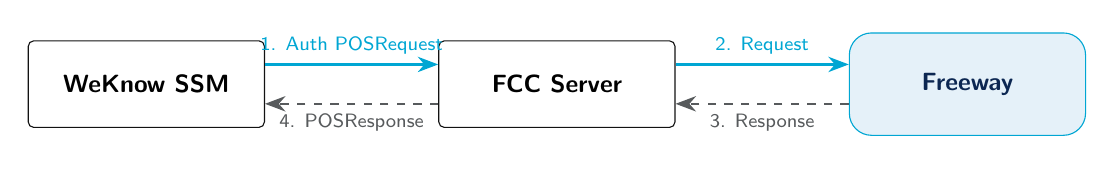
\begin{tikzpicture}[
  box/.style={draw=weknowgraphite,fill=white,rounded corners=2pt,
              minimum width=30mm,minimum height=11mm,align=center,
              font=\small\bfseries},
  cloud/.style={draw=weknowazure,fill=weknowsky,rounded corners=8pt,
              minimum width=30mm,minimum height=13mm,align=center,
              font=\small\bfseries,text=weknownight},
  arr/.style={-{Stealth[length=2.6mm]},thick,weknowazure,font=\scriptsize},
  ret/.style={-{Stealth[length=2.6mm]},thick,dashed,weknowgreyN,font=\scriptsize}]
  \node[box] (ssm) {WeKnow SSM};
  \node[box,right=22mm of ssm] (srv) {FCC Server};
  \node[cloud,right=22mm of srv] (fwy) {Freeway};
  \draw[arr] ([yshift=2.5mm]ssm.east) -- node[above]{1. Auth POSRequest}
             ([yshift=2.5mm]srv.west);
  \draw[arr] ([yshift=2.5mm]srv.east) -- node[above]{2. Request}
             ([yshift=2.5mm]fwy.west);
  \draw[ret] ([yshift=-2.5mm]fwy.west) -- node[below]{3. Response}
             ([yshift=-2.5mm]srv.east);
  \draw[ret] ([yshift=-2.5mm]srv.west) -- node[below]{4. POSResponse}
             ([yshift=-2.5mm]ssm.east);
\end{tikzpicture}
\caption{Card-not-present Auth: the FCC Server talks directly to Freeway; no device interaction.}
\end{figure}

\subsection{Follow-up transactions --- Capture \& follow-on Auth}

Follow-up transactions (Capture, incremental / follow-on authorisations)
reference the original \texttt{RequestID} and are processed
\textbf{direct to Freeway} through the FCC Server; no card interaction is
required.

\begin{figure}[H]
\centering
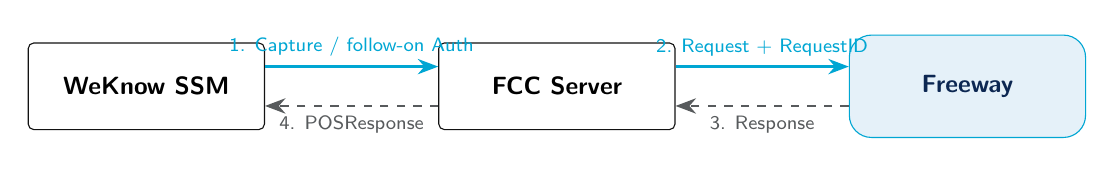
\begin{tikzpicture}[
  box/.style={draw=weknowgraphite,fill=white,rounded corners=2pt,
              minimum width=30mm,minimum height=11mm,align=center,
              font=\small\bfseries},
  cloud/.style={draw=weknowazure,fill=weknowsky,rounded corners=8pt,
              minimum width=30mm,minimum height=13mm,align=center,
              font=\small\bfseries,text=weknownight},
  arr/.style={-{Stealth[length=2.6mm]},thick,weknowazure,font=\scriptsize},
  ret/.style={-{Stealth[length=2.6mm]},thick,dashed,weknowgreyN,font=\scriptsize}]
  \node[box] (ssm) {WeKnow SSM};
  \node[box,right=22mm of ssm] (srv) {FCC Server};
  \node[cloud,right=22mm of srv] (fwy) {Freeway};
  \draw[arr] ([yshift=2.5mm]ssm.east) --
       node[above]{1. Capture / follow-on Auth} ([yshift=2.5mm]srv.west);
  \draw[arr] ([yshift=2.5mm]srv.east) --
       node[above]{2. Request + RequestID} ([yshift=2.5mm]fwy.west);
  \draw[ret] ([yshift=-2.5mm]fwy.west) --
       node[below]{3. Response} ([yshift=-2.5mm]srv.east);
  \draw[ret] ([yshift=-2.5mm]srv.west) --
       node[below]{4. POSResponse} ([yshift=-2.5mm]ssm.east);
\end{tikzpicture}
\caption{Capture and follow-on Auth reference the original RequestID and go direct to Freeway.}
\end{figure}

\begin{wkinfo}[Incremental authorisation mode]
Incremental authorisations are configured as \textbf{adjustments} via
\texttt{incrementalAuthType} in
\texttt{FreewayServerService.exe.config} --- see \S\ref{sec:incremental}.
\end{wkinfo}

%=====================================================================
% 3  SETUP / CONFIGURATION
%=====================================================================
\clearpage
\section{Setup / Configuration}

To complete the connection to FreedomPay in WeKnow, the property's
FreedomPay \textbf{Store ID} and \textbf{Terminal ID} supplied by the
FreedomPay boarding team will be required.

\subsection{FreedomPay Device Management Portal (DMP) Activation Key}

A DMP Activation Key is required for each FCC installation. The key links
the FCC instance with the FreedomPay Enterprise Portal.

\begin{enumerate}
  \item Log into
        \href{https://enterprise-services.freedompay.com/authservices/Account/Login}
        {FreedomPay's Enterprise Portal} using the property's Enterprise
        Code, Username and Password provided by the FreedomPay boarding
        team, and select \textbf{Login}.
\end{enumerate}

\screenshot[0.98]{fp-portal-login}{FreedomPay Enterprise Portal sign-in: enter the Enterprise Code, User Name and Password supplied by the boarding team.}

\begin{enumerate}\setcounter{enumi}{1}
  \item Navigate to \textbf{Device Management} in the toolbar menu and
        select \textbf{Activation Keys}.
\end{enumerate}

\screenshot[0.98]{fp-portal-devicemgmt}{Device Management menu --- select \textbf{Activation Keys}.}

\begin{enumerate}\setcounter{enumi}{2}
  \item Select \textbf{Generate}.
\end{enumerate}

\screenshot[0.98]{fp-portal-generate}{The Activation Keys list --- select \textbf{Generate} to create a new key.}

\begin{enumerate}\setcounter{enumi}{3}
  \item Select \textbf{Copy} (or display the key as a QR code via the
        Action button) and securely store the generated DMP Activation
        Key for use during the FCC installation (\S\ref{sec:install}).
\end{enumerate}

\screenshot[0.98]{fp-portal-copykey}{Use the \textbf{Copy} action to capture the generated key. (Key values are redacted here.)}

\subsection{Network requirements --- Windows FCC}\label{sec:network}

A network administrator must complete port forwarding on the local
network router to port \textbf{1011} (HTTP) or \textbf{1013} (HTTPS) and
provide a static IP address for the FCC workstation; this address is used
as the FCC Server URL in WeKnow. All outbound traffic to FreedomPay is
\textbf{HTTPS on port 443 using TLS 1.2 or higher}.

\subsubsection*{Outbound allow-list (firewall)}

\begin{center}
\renewcommand{\arraystretch}{1.3}\small
\begin{tabularx}{\textwidth}{L{20mm} X X}
\rowcolor{weknownight}\color{white}\textbf{Environment} &
\color{white}\textbf{FreedomPay IP ranges} &
\color{white}\textbf{Domain names}\\
\textbf{Production} &
64.74.156.0/24\newline 52.177.83.208/32\newline 91.195.241.0/24 &
cs.freedompay.us\newline manager.freedompay.us\newline
enterprise-services.freedompay.com\newline cdn.freedompay.com\\
\rowcolor{weknowgreyL}
\textbf{UAT (Test)} &
20.15.0.240/28\newline 20.15.1.0/28\newline 20.44.79.130/32\newline
20.85.63.144/28\newline 20.96.246.128/28\newline
20.96.247.32/28\newline 40.65.212.0/28 &
cs.uat.freedompay.com\newline manager.uat.freedompay.com\newline
enterprise-services.uat.freedompay.com\newline cdn.uat.freedompay.com\\
\end{tabularx}
\end{center}

\subsubsection*{Endpoint URLs and ports}

\begin{center}
\renewcommand{\arraystretch}{1.3}\small
\begin{tabularx}{\textwidth}{L{18mm} X L{20mm} L{24mm}}
\rowcolor{weknownight}\color{white}\textbf{Platform} &
\color{white}\textbf{URLs} &
\color{white}\textbf{Outbound port} &
\color{white}\textbf{Inbound ports}\\
\textbf{Live} &
{\scriptsize\ttfamily
https://cs.freedompay.us/Freeway/Service.asmx\newline
https://cs.freedompay.us/CardStor/CardStorService.asmx\newline
https://manager.freedompay.us/DCC/HFEX.txt\newline
https://manager.freedompay.us/Map/BinMap2.txt\newline
https://enterprise-services.freedompay.com/\newline
\hspace*{3mm}AssetManagement/api/v2/\newline
https://enterprise-services.freedompay.com/\newline
\hspace*{3mm}AuthorizationServer/auth/activationkeys/}
& 443 & 1011, 1012, 1013, 3391, 3392, 5015, 5080, 8090\\
\rowcolor{weknowgreyL}
\textbf{Test} &
{\scriptsize\ttfamily
https://cs.uat.freedompay.com/Freeway/Service.asmx\newline
https://cs.uat.freedompay.com/CardStor/CardStorService.asmx\newline
https://manager.uat.freedompay.com/DCC/HFEX.txt\newline
https://manager.uat.freedompay.com/Map/BinMap2.txt\newline
https://enterprise-services.uat.freedompay.com/\newline
\hspace*{3mm}AssetManagement/api/v2/\newline
https://enterprise-services.uat.freedompay.com/\newline
\hspace*{3mm}AuthorizationServer/auth/activationkeys/}
& 443 & 1011, 1012, 1013, 3340, 3391, 3392, 5015, 5080, 8090\\
\end{tabularx}
\end{center}

\begin{wkwarn}[Port reference (FCC Server defaults)]
\texttt{xmlPort} 1011 (XML POSRequests, used by WeKnow),
\texttt{nvpPort} 1012, \texttt{sslXmlPort} 1013,
\texttt{clientPort} 3391 (FCC Client to Server),
\texttt{TLSSusannaConnection.clientPort} 3392,
\texttt{httpProxyPort} 5080. Always check the current FCC documentation
at \url{https://docs.freedompay.com} for the latest values.
\end{wkwarn}

\subsection{Install the FCC Client (Standalone)}\label{sec:install}

\begin{wkinfo}[Where to get the installer]
Download the FCC installation package
(\texttt{FCC\_5.4.3.20.zip} or later) and the WeKnow UAT configuration
bundle from the internal WeKnow mirror:\\
{\ttfamily https://dev.weknowlondon.uk/SSM/freedompay/}\\
The current release is also published on FreedomPay's documentation
portal (FCC $\rightarrow$ Setup $\rightarrow$ Installation $\rightarrow$
Standalone). \textbf{Minimum supported version for WeKnow is FCC
5.4.x.} Do not deploy the legacy 5.3.2.15 package.
\end{wkinfo}

\begin{enumerate}
  \item Connect the EFTPOS terminal to the WeKnow workstation using the
        provided USB cable.
  \item Unzip the installation package. The extracted \texttt{DISK1}
        folder contains the installer and the configuration files edited
        in \S\ref{sec:config}.
\end{enumerate}

\screenshot[0.86]{fcc-folder-serverconfig}{Extracted \texttt{DISK1} folder --- the installer (\texttt{FreewayCommerceConnect}) sits alongside the \texttt{.config} files.}

\begin{enumerate}\setcounter{enumi}{2}
  \item Right-click \texttt{FreewayCommerceConnect.exe} and select
        \textbf{Run as administrator}. Choose \textbf{Run Anyway} on any
        Windows SmartScreen prompt.
\end{enumerate}

\screenshot[0.72]{fcc-run-as-admin}{Launch the installer with \textbf{Run as administrator}.}

\begin{enumerate}\setcounter{enumi}{3}
  \item The \textbf{Remote Update Service (RUS)} setup launches first.
        Click \textbf{Next}.
\end{enumerate}

\screenshot[0.56]{fcc-rus-welcome}{Remote Update Service setup wizard --- click \textbf{Next} to begin.}

\begin{enumerate}\setcounter{enumi}{4}
  \item Enter the field information:
    \begin{itemize}
      \item \textbf{DMP Activation URL} --- defaults to Production. For a
            UAT install, overwrite with the UAT URL (table below).
      \item \textbf{DMP Activation Key} --- the key generated in the
            Enterprise Portal.
      \item \textbf{Proxy Activation URL} --- leave blank unless the
            workstation lacks direct internet access (contact the
            FreedomPay SI team for the proxy URL if required).
    \end{itemize}
\end{enumerate}

\screenshot[0.56]{fcc-rus-url}{Device Management Portal Activation URL --- defaults to Production; replace with the UAT URL for a test install.}

\screenshot[0.56]{fcc-rus-key}{Enter the DMP Activation Key generated in the Enterprise Portal, then click \textbf{Next}.}

\begin{enumerate}\setcounter{enumi}{5}
  \item Click \textbf{Next}, then \textbf{Finish} to complete the RUS
        setup.
  \item The FCC installer welcome screen appears. Click \textbf{Next},
        then choose the Setup Type.
  \item Choose Setup Type \textbf{Typical} and click \textbf{Next}.
\end{enumerate}

\screenshot[0.56]{fcc-setup-type}{Choose \textbf{Typical} for a standard WeKnow standalone install.}

\begin{wkinfo}[When to choose Custom]
Select \textbf{Custom} only if instructed --- for example to add the
\emph{FCC Test Client} transaction simulator for UAT testing, or to
deselect the \emph{FCC Client User Interface} when the on-screen payment
status should not be displayed.
\end{wkinfo}

\screenshot[0.56]{fcc-custom-setup}{Custom Setup feature tree --- tick \emph{FCC Test Client} for UAT simulation; leave defaults otherwise.}

\begin{enumerate}\setcounter{enumi}{8}
  \item Click \textbf{Finish}. The FCC Server Service and FCC Client
        Service are installed and started.
\end{enumerate}

\begin{center}
\renewcommand{\arraystretch}{1.3}\small
\begin{tabularx}{\textwidth}{L{22mm} X}
\rowcolor{weknownight}\color{white}\textbf{Environment} &
\color{white}\textbf{DMP Activation URL}\\
Production & \scriptsize\ttfamily
https://enterprise-services.freedompay.com/authorizationserver/auth/activationkeys/\\
\rowcolor{weknowgreyL}
UAT & \scriptsize\ttfamily
https://enterprise-services.uat.freedompay.com/authorizationserver/auth/activationkeys/\\
\end{tabularx}
\end{center}

\subsubsection*{Installed file locations}

\begin{center}
\renewcommand{\arraystretch}{1.3}\small
\begin{tabularx}{\textwidth}{L{34mm} X}
\rowcolor{weknownight}\color{white}\textbf{Purpose} &
\color{white}\textbf{Path}\\
Binaries \& config files &
\ttfamily C:\textbackslash Program Files (x86)\textbackslash
FreedomPay\textbackslash FreewayCommerceConnect\\
\rowcolor{weknowgreyL}
Logs & \ttfamily C:\textbackslash ProgramData\textbackslash
FreedomPay\textbackslash Freeway Commerce Connect\textbackslash log\\
PAL packages & \ttfamily C:\textbackslash ProgramData\textbackslash
FreedomPay\textbackslash Freeway Commerce Connect\textbackslash pal\\
\end{tabularx}
\end{center}

\begin{wkwarn}[Hidden folder]
\texttt{ProgramData} is hidden by Windows by default. Paste the path
directly into the File Explorer address bar if it is not visible.
\end{wkwarn}

\subsection{Configuration files}\label{sec:config}

FCC behaviour is controlled by five files in the installation folder.
\textbf{After changing any config file, restart the corresponding Windows
service} (Windows Services app $\rightarrow$ right-click
\emph{Freeway Server Service} / \emph{Freeway Client Service}
$\rightarrow$ \textbf{Restart}).

\begin{center}
\renewcommand{\arraystretch}{1.3}\small
\begin{tabularx}{\textwidth}{L{52mm} X}
\rowcolor{weknownight}\color{white}\textbf{File} &
\color{white}\textbf{Controls}\\
\ttfamily AMA.config & Asset Management / DMP endpoints (v2 API).\\
\rowcolor{weknowgreyL}
\ttfamily FreewayServerService.exe.config &
Server-side processing: ports, Freeway URLs, Store-and-Forward
(offline), receipts, incremental auth.\\
\ttfamily FreewayClientService.exe.config &
Client-side behaviour: Freeway/CardStor URLs, device types, DCC,
logging, PAL.\\
\rowcolor{weknowgreyL}
\ttfamily LaneConfig.xml &
Maps the logical lane to the physical POI device (serial number for
USB).\\
\ttfamily Servers.xml &
Client-to-Server routing. \textbf{No change needed for standalone
installations.}\\
\end{tabularx}
\end{center}

\subsubsection{Offline accept (Store-and-Forward)}

The \texttt{floorLimit} key in \texttt{FreewayServerService.exe.config}
controls offline acceptance. The FCC ships with a default of
\texttt{50}; \textbf{WeKnow policy is to disable offline acceptance}, so
set the value to \texttt{0}:

\begin{lstlisting}
<!-- floor limit - maximum amount accepted in an Offline Accept -->
<add key="floorLimit" value="0" />
\end{lstlisting}

How Store-and-Forward behaves when a non-zero floor limit is configured:
if the FCC cannot contact Freeway (or Freeway cannot contact the
processor) and the amount requested is below the floor limit, the FCC
stores the request and replays it periodically. The retry frequency is
set by \texttt{saf.replayInterval} (default: every 5 minutes). If Freeway
declines the replay, the FCC retries once a day
(\texttt{saf.RejectReplayTimer}, default 1440 minutes) in the hope funds
become available, accepting partial payment where offered. After
\texttt{offlineMaxDays} (default 30, maximum 60) an authorisation is no
longer valid, the request is marked declined, and \textbf{the merchant
bears the loss} --- which is why WeKnow keeps the floor limit at 0.

\subsubsection{Regional configuration}

Set the locale keys in \textbf{both} config files to match the property's
region, then restart both services.

\paragraph{1. United States}
\begin{lstlisting}
<!-- FreewayServerService.exe.config -->
<add key="baseCulture" value="en-US" />
<add key="receiptFormatter" value="us" />
<add key="merchantCurrencyCode" value="USD" />

<!-- FreewayClientService.exe.config -->
<add key="dcc.LocalCurrency" value="USD" />
<add key="dcc.LocalCurrencyCode" value="840" />
\end{lstlisting}

\paragraph{2. United Kingdom}
\begin{lstlisting}
<!-- FreewayServerService.exe.config -->
<add key="baseCulture" value="en-GB" />
<add key="receiptFormatter" value="uk" />
<add key="merchantCurrencyCode" value="GBP" />

<!-- FreewayClientService.exe.config -->
<add key="dcc.LocalCurrency" value="GBP" />
<add key="dcc.LocalCurrencyCode" value="826" />
\end{lstlisting}

\paragraph{3. European Union}
\begin{lstlisting}
<!-- FreewayServerService.exe.config -->
<add key="baseCulture" value="de-DE" />
<add key="receiptFormatter" value="europe" />
<add key="merchantCurrencyCode" value="EUR" />

<!-- FreewayClientService.exe.config -->
<add key="dcc.LocalCurrency" value="EUR" />
<add key="dcc.LocalCurrencyCode" value="978" />
\end{lstlisting}

\begin{wkwarn}[UK deployments --- signature validation]
Where the signature Card Verification Method applies (attended lanes),
WeKnow SSM must validate the receipt signature against the card. On a
mismatch, SSM must immediately send a \textbf{Void} request to the FCC to
nullify the transaction and release the cardholder's funds.
\end{wkwarn}

\subsubsection{Lane configuration (POI device)}

Open \texttt{LaneConfig.xml} and enter the EFTPOS terminal's serial
number for the USB-connected lane, then save the file:

\begin{lstlisting}
<laneConfigMap>
  <lanes>
    <lane id="1" deviceTerminalId="FP000001" serialNumber="<terminal serial>" />
  </lanes>
</laneConfigMap>
\end{lstlisting}

\subsubsection{Device type (kernel setting)}

In \texttt{FreewayClientService.exe.config}, set the kernel device types
for the deployed terminals. WeKnow production values:

\begin{lstlisting}
<!-- Telium devices ('rba', 'ram', 'cpx') -->
<add key="teliumDefaultDeviceType" value="rba" />
<!-- Tetra devices e.g. Lane 3000 / 3600 ('ram', 'upp') -->
<add key="tetraDefaultDeviceType" value="upp" />
\end{lstlisting}

After editing and saving, restart the Freeway Client Service and the
WeKnow SSM.

\subsubsection{Incremental authorisation (Adjustment)}\label{sec:incremental}

In \texttt{FreewayServerService.exe.config}, WeKnow runs incremental
authorisations as \textbf{adjustments}:

\begin{lstlisting}
<!-- Valid values: reauth | adjustment | reauthorize -->
<add key="incrementalAuthType" value="adjustment" />
\end{lstlisting}

\subsection{Switching between UAT and Production}

The FCC environment is determined by the Freeway / CardStor URLs in both
config files \textbf{and} the DMP endpoints in \texttt{AMA.config}. Keep
all endpoints in the \emph{same} environment --- never mix UAT and
Production.

\paragraph{FreewayServerService.exe.config}
\begin{lstlisting}
<!-- UAT -->
<add key="freewayServer" value="https://cs.uat.freedompay.com/" />
<add key="cardStorUrl"
     value="https://cs.uat.freedompay.com/CardStor/CardStorService.asmx" />

<!-- Production -->
<add key="freewayServer" value="https://cs.freedompay.us/" />
<add key="cardStorUrl"
     value="https://cs.freedompay.us/CardStor/CardStorService.asmx" />
\end{lstlisting}

\paragraph{FreewayClientService.exe.config}
\begin{lstlisting}
<!-- UAT -->
<add key="freewayUrl"
     value="https://cs.uat.freedompay.com/Freeway/Service.asmx" />
<add key="cardStorUrl"
     value="https://cs.uat.freedompay.com/CardStor/CardStorService.asmx" />

<!-- Production -->
<add key="freewayUrl"
     value="https://cs.freedompay.us/Freeway/Service.asmx" />
<add key="cardStorUrl"
     value="https://cs.freedompay.us/CardStor/CardStorService.asmx" />
\end{lstlisting}

\paragraph{AMA.config}
\begin{lstlisting}
<!-- UAT -->
<assetManagementSettings
  baseUrl="https://enterprise-services.uat.freedompay.com/
           AssetManagement/api/v2/"
  activationUrl="https://enterprise-services.uat.freedompay.com/
           AuthorizationServer/auth/activationkeys/">
</assetManagementSettings>
<!-- (URLs shown wrapped for print; enter each as a single line) -->
\end{lstlisting}

Save the changes and \textbf{restart both Freeway services}. The FCC
Client can also be re-pointed by opening the FCC Client, selecting
\textbf{Configure}, and replacing the DMP Activation URL with the URL for
the required environment.

\begin{wkwarn}[Common pitfall]
Note the domain difference: Production Freeway is
\texttt{cs.freedompay.\textbf{us}}, UAT is
\texttt{cs.uat.freedompay.\textbf{com}}. Mixing \texttt{.us}/\texttt{.com}
is the most frequent cause of error 234 (invalid merchant credentials)
and 3042 (exceeds max days offline).
\end{wkwarn}

\subsection{PAL package updates (device firmware \& configuration)}

Lane 3000 / Lane 3600 devices used in production periodically need
firmware or configuration updates to comply with new card-brand mandates
or to address security issues. Packages are pushed via the \textbf{PAL}
(Payment Application Loader) subsystem built into the Windows FCC.

\subsubsection*{Obtaining packages}

Current PAL packages for WeKnow terminals are maintained on the internal
mirror (\url{https://dev.weknowlondon.uk/SSM/freedompay/}) and are
kept up to date from FreedomPay update notifications. Packages can also
be uploaded, published and pushed remotely from the Enterprise Portal
(\textbf{Device Management $\rightarrow$ PAL Packages}: Upload
$\rightarrow$ complete the PAL Details form $\rightarrow$
\textbf{Publish}).

\subsubsection*{Local push procedure}

\begin{enumerate}
  \item Download the required packages for the device.
  \item Copy the \texttt{.palpkg} files into:\newline
        {\ttfamily C:\textbackslash ProgramData\textbackslash
        FreedomPay\textbackslash Freeway Commerce
        Connect\textbackslash pal}
  \item Edit \texttt{profile.dat} in the same folder so it lists exactly
        the packages to apply, for example:
\begin{lstlisting}
firmware.{devtype}
baseconfig.{devtype}
\end{lstlisting}
  \item Save \texttt{profile.dat}. The PAL subsystem performs a periodic
        check every \texttt{palCheckInterval} minutes (default 5) and a
        forced check on service start-up or new device detection.
  \item To force an immediate push, restart the Freeway Client Service,
        or reset the POI device (press and hold \textbf{\#} and the
        \textbf{yellow} button together until the device resets).
  \item Watch the device: \texttt{firmware.ogz} or \texttt{config.tgz}
        on-screen means the package is transferring. The device may
        reboot one or more times; leave it connected until activity
        stops and it returns to the \emph{secured by freedompay} screen
        for about a minute. The device is then ready for use.
\end{enumerate}

\begin{wkinfo}[Scheduled pushes]
Packages flagged \texttt{scheduled=1} are only pushed during the
configured off-hours window (\texttt{offHoursStart}=11pm to
\texttt{offHoursEnd}=4am by default), so device updates do not interrupt
trading.
\end{wkinfo}

\subsection{Setup Payment Gateway in WeKnow}

\begin{enumerate}
  \item In the WeKnow website, go to \textbf{Others $\rightarrow$ Masters
        $\rightarrow$ Payment Gateway Setup}.
\end{enumerate}

\screenshot[0.98]{weknow-gateway-setup}{WeKnow Payment Gateway Setup --- select FreedomPay and enter the FCC Server URL, Store ID and Terminal ID. (Credentials redacted.)}

\begin{enumerate}\setcounter{enumi}{1}
  \item Enter the \textbf{FCC Server URL}: the static IP address of the
        FCC workstation, ending in port \textbf{1011} (HTTP) or
        \textbf{1013} (HTTPS), e.g.\
        {\ttfamily http://192.168.1.50:1011}.
  \item Enter the FreedomPay \textbf{Store ID} and \textbf{Terminal ID}.
\end{enumerate}

\subsubsection*{Credential storage}

\begin{itemize}
  \item Store ID and Terminal ID are stored as \textbf{encrypted data}.
  \item Data is carried in an encrypted format end-to-end.
  \item Data is decrypted dynamically only at the moment an FCC request
        is made.
\end{itemize}

%=====================================================================
% 4  LEVEL 1 TROUBLESHOOTING GUIDE
%=====================================================================
\clearpage
\section{Level 1 Troubleshooting Guide}

Responses from Freeway always include an \texttt{errorCode}, which
WeKnow displays to the operator. Code \textbf{100 = Approved}; anything
else raises an alert in the WeKnow UI. This section equips WeKnow L1
support to interpret the most common codes and resolve them --- or
collect the right evidence before escalating to FreedomPay.

\begin{figure}[H]
\centering
\setlength{\fboxsep}{0pt}\setlength{\fboxrule}{0.6pt}%
{\color{weknowgreyM}\fbox{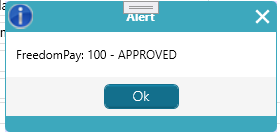
\includegraphics[width=0.30\linewidth]{weknow-txn-approved}}}\hfill
{\color{weknowgreyM}\fbox{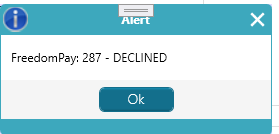
\includegraphics[width=0.30\linewidth]{weknow-txn-error}}}\hfill
{\color{weknowgreyM}\fbox{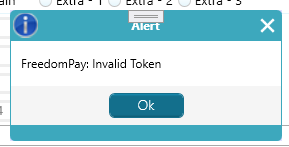
\includegraphics[width=0.30\linewidth]{weknow-txn-decline}}}
\caption{Example Freeway responses as shown to the WeKnow operator: an approval (100), a decline (287) and a validation error (invalid token).}
\end{figure}

\subsection{Before anything else --- two preliminary checks}

\begin{enumerate}
  \item \textbf{Environment alignment.} Confirm every configured endpoint
        (Freeway, CardStor, AMA) matches the intended environment. UAT
        credentials against Production URLs (or vice versa) cause most
        credential and offline errors.
  \item \textbf{Connectivity integrity.} Verify DNS resolution, firewall
        rules (\S\ref{sec:network}), proxy settings and TLS-inspection
        exclusions for the FreedomPay domains.
\end{enumerate}

\begin{wkwarn}[After any config change]
Restart the Freeway Server Service and Freeway Client Service via the
Windows Services application. Config changes do not take effect until
the services restart.
\end{wkwarn}

\subsection{Common error codes and remediation}

\textbf{Worked example.} A transaction returns
\emph{``234: Invalid merchant credentials''}. First check the Store ID /
Terminal ID configured in WeKnow Payment Gateway Setup. If they are
correct, confirm the FCC URLs point at the same environment as the
credentials (\texttt{.us} = Production, \texttt{uat...com} = UAT). If the
error persists, escalate to FreedomPay.

\begin{center}
\renewcommand{\arraystretch}{1.35}\small
\begin{tabularx}{\textwidth}{L{12mm} L{44mm} X}
\rowcolor{weknownight}\color{white}\textbf{Code} &
\color{white}\textbf{Meaning} & \color{white}\textbf{L1 action}\\
100 & Approved & Success --- no action.\\
\rowcolor{weknowgreyL}
101 / 102 & Required field missing / invalid data &
Check \texttt{missingFields} / \texttt{invalidFields} in the response
(e.g.\ \texttt{invoiceNumber} $>$ 20 characters). Escalate to WeKnow
engineering --- usually needs a code change.\\
104 & Duplicate transaction & Contact FreedomPay Tech Support.\\
\rowcolor{weknowgreyL}
201--221 & Issuer declines (expired card, insufficient funds, incorrect
PIN/CVV, etc.) & Follow the \texttt{decision} field; retry with the
customer where appropriate. No system fault.\\
217 & Soft decline / additional authentication &
Contactless: ask the customer to insert and enter PIN.\\
\rowcolor{weknowgreyL}
234 & Invalid merchant credentials &
Verify Store ID / Terminal ID in WeKnow; verify FCC URLs match the
environment; then contact FreedomPay.\\
250 / 252 & Processor timeout / unavailable &
Wait and retry; check \url{https://status.freedompay.com}.\\
\rowcolor{weknowgreyL}
261 & Track-data decryption error &
Usually a device with the wrong environment encryption keys (UAT device
in Production or vice versa). Email FreedomPay Systems Integrations with
the FCC Client log.\\
3001 & Freeway connection error &
Network failure between FCC and Freeway. Check connectivity/firewall;
review logs.\\
\rowcolor{weknowgreyL}
3005 / 3019 & Request ID not found &
The follow-on referenced a \texttt{RequestID} unknown to FCC. Verify the
original transaction; review logs.\\
3021 / 3022 & Offline accept / decline &
FCC is offline. Verify endpoints and network reachability; review logs
around the event window. (WeKnow sets \texttt{floorLimit}=0, so offline
accepts should not occur in production.)\\
\rowcolor{weknowgreyL}
3030 / 3034 & Lane / FCC Client timeout &
Customer did not present a card in time, or the Client did not respond.
Retry; check device and Client service status.\\
3042 & Exceeds max days offline &
After a stable deployment this almost always means \textbf{incorrect
Freeway URLs} (check \texttt{.us} vs \texttt{.com}). Fix endpoints,
restore connectivity, restart services.\\
\rowcolor{weknowgreyL}
3120 / 3128 & No device / device timeout &
Check the USB connection and the serial number in
\texttt{LaneConfig.xml}; power-cycle the POI device.\\
3133 & User cancel & Customer pressed cancel --- retry the payment.\\
\end{tabularx}
\end{center}

The complete, current list is maintained at
\url{https://docs.freedompay.com/fcc/response-codes/error-codes}.

\subsection{Log collection}

FCC logs live in:\newline
{\ttfamily C:\textbackslash ProgramData\textbackslash
FreedomPay\textbackslash Freeway Commerce Connect\textbackslash log}

The FCC Client verbosity is set with \texttt{logLevel} in
\texttt{FreewayClientService.exe.config}. Levels, in order of verbosity:

\begin{itemize}
  \item \textbf{Critical} --- only fatal issues.
  \item \textbf{Error} --- significant errors that don't crash the app.
  \item \textbf{Warning} --- non-critical issues worth noting.
  \item \textbf{Information} --- general operational entries.
  \item \textbf{Verbose} --- detailed logs of normal operations.
  \item \textbf{Debug1--Debug4} --- increasing debug detail; Debug4 is
        the most detailed (method entry/exit, variable states, etc.).
        Use Debug levels in UAT; production typically runs at
        Information/Verbose.
\end{itemize}

If L1 cannot access the workstation remotely, ask the site contact to
zip the entire \texttt{log} folder (logs auto-compress after 7 days and
are retained 30 days by default) and attach it to the support ticket.

\subsection{Escalating to FreedomPay}

FreedomPay provides \textbf{Level 2+ technical support}, 24/7/365 for
production issues, for faults triaged by WeKnow L1 as originating in the
FreedomPay ecosystem (Freeway, FCC, or hardware).

\begin{center}
\renewcommand{\arraystretch}{1.3}\small
\begin{tabularx}{\textwidth}{L{34mm} X}
\rowcolor{weknownight}\color{white}\textbf{Channel} &
\color{white}\textbf{Contact}\\
Phone (US) & 888\,495\,2446\\
\rowcolor{weknowgreyL}
Phone (UK) & +44\,203\,014\,8966\\
Email & techsupport@freedompay.com\\
\rowcolor{weknowgreyL}
Status page & \url{https://status.freedompay.com} (subscribe to updates)\\
\end{tabularx}
\end{center}

\subsubsection*{Pre-contact checklist --- include with every ticket}

\begin{itemize}
  \item[$\square$] Confirmation that WeKnow L1 troubleshooting steps have
        been exhausted.
  \item[$\square$] Clear description of current vs.\ expected behaviour.
  \item[$\square$] Integration details: POS = WeKnow SSM; integration
        type = \textbf{Windows FCC}.
  \item[$\square$] Relevant \textbf{RequestIDs} and the exact
        \textbf{error codes} received.
  \item[$\square$] FCC Client and Server \textbf{logs} and \textbf{config
        files}, ideally including a fresh service restart captured in the
        logs.
  \item[$\square$] Workstation name as it appears in the Enterprise
        Portal, and the raw \texttt{POSRequest} where available.
\end{itemize}

\subsubsection*{FreedomPay priority levels \& response SLAs}

\begin{center}
\renewcommand{\arraystretch}{1.3}\small
\begin{tabularx}{\textwidth}{L{24mm} X L{28mm}}
\rowcolor{weknownight}\color{white}\textbf{Priority} &
\color{white}\textbf{Description / example} &
\color{white}\textbf{Response SLA}\\
P1 -- Critical & Business-critical services down, no workaround
(total store outage). & 30 minutes\\
\rowcolor{weknowgreyL}
P2 -- High & Restricted/degraded service for a large segment
(multiple device failures, heavy latency). & 4 hours\\
P3 -- Medium & Partial or non-critical loss (refunds, batching,
settlement queries). & 2 business days\\
\rowcolor{weknowgreyL}
P4 -- Low & General usage/reporting questions, documentation
requests. & 3 business days\\
\end{tabularx}
\end{center}

\subsection{Escalation flow at a glance}

\begin{figure}[H]
\centering
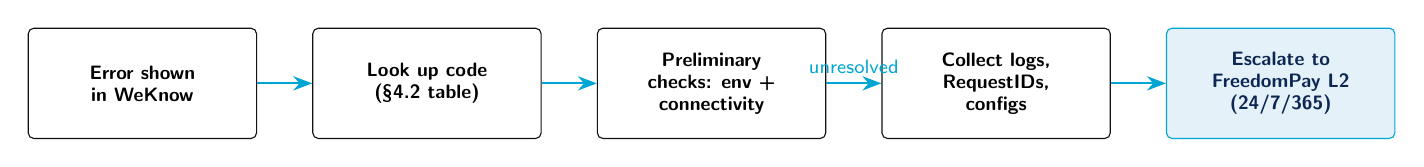
\begin{tikzpicture}[
  fstep/.style={draw=weknowgraphite,fill=white,rounded corners=2pt,
               minimum width=29mm,minimum height=14mm,align=center,
               font=\scriptsize\bfseries},
  hot/.style={draw=weknowazure,fill=weknowsky,rounded corners=2pt,
               minimum width=29mm,minimum height=14mm,align=center,
               font=\scriptsize\bfseries,text=weknownight},
  arr/.style={-{Stealth[length=2.4mm]},thick,weknowazure,font=\scriptsize}]
  \node[fstep] (a) {Error shown\\in WeKnow};
  \node[fstep,right=7mm of a] (b) {Look up code\\(\S 4.2 table)};
  \node[fstep,right=7mm of b] (c) {Preliminary\\checks: env +\\connectivity};
  \node[fstep,right=7mm of c] (d) {Collect logs,\\RequestIDs,\\configs};
  \node[hot,right=7mm of d] (e) {Escalate to\\FreedomPay L2\\(24/7/365)};
  \draw[arr] (a) -- (b);
  \draw[arr] (b) -- (c);
  \draw[arr] (c) -- node[above]{unresolved} (d);
  \draw[arr] (d) -- (e);
\end{tikzpicture}
\caption{WeKnow L1 triage path, ending in escalation to FreedomPay Level 2 support.}
\end{figure}

%=====================================================================
% APPENDIX
%=====================================================================
\clearpage
\section*{Appendix --- Reference documents}
\addcontentsline{toc}{section}{Appendix --- Reference documents}

\begin{itemize}
  \item FreedomPay documentation portal (FCC | Windows):
        \url{https://docs.freedompay.com/fcc/welcome/readme}
  \item FCC error codes \& troubleshooting:
        \url{https://docs.freedompay.com/fcc/response-codes/error-codes}
  \item FCC configuration file reference:
        \url{https://docs.freedompay.com/fcc/setup/files}
  \item Production go-live \& technical support:\newline
        {\small\url{https://docs.freedompay.com/production-go-live-guide/post-launch/technical-support}}
  \item FreedomPay service status: \url{https://status.freedompay.com}
  \item Internal WeKnow mirror (installers, PAL packages, guides):
        {\ttfamily https://dev.weknowlondon.uk/SSM/freedompay/}
  \item Freeway Commerce Connect API Guide, DCC Configuration Guide, PAL
        Package Deployment Guide --- see the internal mirror above.
\end{itemize}

\vspace{12mm}
\begin{center}

\includegraphics[width=42mm]{wkg-logo-stacked}\\[5mm]
{\color{weknowgreyN}\small
For questions about this document contact WeKnow Integrations.\\
For WeKnow branding queries contact louise.vineeta@weknowgroup.com}
\end{center}

\end{document}
